\documentclass[twocolumn,a4paper]{article}
\usepackage{fontspec}   %加這個就可以設定字體
\usepackage{xeCJK}       %讓中英文字體分開設置
\usepackage{indentfirst}
\usepackage{listings}
\usepackage[newfloat]{minted}
\usepackage{float}
\usepackage{graphicx}
\usepackage{caption}
\usepackage{fancyhdr}
\usepackage{hyperref}
\usepackage{amsmath}
\usepackage{multirow}
\usepackage[dvipsnames]{xcolor}
\usepackage{graphicx}
\usepackage{tabularx}
\usepackage{booktabs}
\usepackage{caption}
\usepackage{subcaption}
\usepackage{pifont}
\usepackage{amssymb}
\usepackage[backend=biber]{biblatex}
\addbibresource{main.bib}


\usepackage{pdftexcmds}
\usepackage{catchfile}
\usepackage{ifluatex}
\usepackage{ifplatform}

\usepackage[breakable, listings, skins, minted]{tcolorbox}
\usepackage{etoolbox}
\setminted{fontsize=\footnotesize}
\renewtcblisting{minted}{%
    listing engine=minted,
    minted language=python,
    listing only,
    breakable,
    enhanced,
    minted options = {
        linenos, 
        breaklines=true, 
        breakbefore=., 
        % fontsize=\footnotesize, 
        numbersep=2mm
    },
    overlay={%
        \begin{tcbclipinterior}
            \fill[gray!25] (frame.south west) rectangle ([xshift=4mm]frame.north west);
        \end{tcbclipinterior}
    }   
}

\usepackage[
top=1.5cm,
bottom=0.75cm,
left=1.5cm,
right=1.5cm,
includehead,includefoot,
heightrounded, % to avoid spurious underfull messages
]{geometry} 

\newenvironment{code}{\captionsetup{type=listing}}{}
\SetupFloatingEnvironment{listing}{name=Code}



\title{Deep Learning Lab 4 - Conditional VAE for Video Prediction}
\author{110550088 李杰穎}
\date{\today}


\setCJKmainfont{Noto Serif TC}



\ifwindows
\setmonofont[Mapping=tex-text]{Consolas}
\fi

\XeTeXlinebreaklocale "zh"             %這兩行一定要加,中文才能自動換行
\XeTeXlinebreakskip = 0pt plus 1pt     %這兩行一定要加,中文才能自動換行

\newcommand*{\dif}{\mathop{}\!\mathrm{d}}


%\setlength{\parindent}{0em}
%\setlength{\parskip}{2em}
%\renewcommand{\baselinestretch}{1.25}
%\setlength{\droptitle}{-7.5em}   % This is your set screw
%\setlength{\columnsep}{2em}

\begin{document}
\maketitle
\section{Introduction}
In this assignment, we implemented and trained a conditional variational autoencoder (cVAE) to predict the next video frame given a previous frame and the next pose image. This architecture follows the approach described in the ICCV paper ``Everybody Dance Now'' \cite{chan2019everybody} and the ICML paper ``Stochastic Video Generation with a Learned Prior'' \cite{denton2018stochastic}, which both address video prediction challenges but in different frameworks (GAN vs. VAE).

The key challenge in video prediction lies in capturing the inherent uncertainty in future frames. Using a conditional VAE allows us to model this uncertainty through a latent space that captures possible motion variations. We trained the model with different KL annealing scheduling strategies, including monotonic, cyclical, and no annealing. The results indicate that cyclical annealing leads to better validation PSNR, which aligns with the findings in \cite{fu2019cyclical} regarding mitigating KL vanishing.

Our best-performing model achieved 38.24 PSNR on the validation set and 36.07 PSNR on the public test set, demonstrating the effectiveness of the proposed approach.

\section{Implementation Details}
\subsection{Model Architecture}

The conditional VAE architecture consists of several key components that work together to generate future video frames based on previous frames and pose information:

\begin{itemize}
    \item \textbf{Frame Encoder (RGB\_Encoder):} Transforms RGB images into feature representations with dimension F\_dim (128)
    \item \textbf{Label Encoder (Label\_Encoder):} Transforms pose images into feature representations with dimension L\_dim (32)
    \item \textbf{Gaussian Predictor:} Models the posterior distribution of latent variables with dimension N\_dim (12)
    \item \textbf{Decoder Fusion:} Combines features from the previous frame, next pose, and sampled latent vector
    \item \textbf{Generator:} Produces the final output frame from the fused representation
\end{itemize}

\paragraph{The \texttt{forward} function.} It takes three inputs: \texttt{img\_prev} (previous frame from ground truth or generated by the model), \texttt{img\_next} (next frame), and \texttt{label\_next} (pose image of next frame). The function encodes the inputs, samples a latent vector, and generates the next frame:

\begin{code}
\captionof{listing}{\textbf{Implementation of the \texttt{forward} function.}}
\label{code:forward}
\begin{minted}
def forward(self, img_prev, img_next, label_next):
    img_prev_encoded = self.frame_transformation(img_prev).detach()  # [batch_size, F_dim]
    img_next_encoded = self.frame_transformation(img_next)  # [batch_size, F_dim]
    label_next_encoded = self.label_transformation(label_next)  # [batch_size, L_dim]

    # Concatenate the transformed image and label
    z, mu, logvar = self.Gaussian_Predictor.forward(img_next_encoded, label_next_encoded)  # [batch_size, N_dim]
    
    # Decoder Fusion
    x = self.Decoder_Fusion.forward(img_prev_encoded, label_next_encoded, z)  # [batch_size, D_out_dim]
    output = self.Generator.forward(x)  # [batch_size, 3, H, W]

    return output, mu, logvar
\end{minted}
\end{code}


\subsection{Training Protocol}
The training protocol follows a conditional VAE framework where the model learns to predict the next frame in a video sequence based on the previous frame and the next pose.

\paragraph{\texttt{training\_stage}.} This method orchestrates the overall training loop. For each epoch, it prepares the training dataloader and determines whether to apply teacher forcing based on a predefined ratio. During the inner loop, it performs forward and backward passes over each batch, accumulating losses.

After each epoch, the method logs averaged loss values to Weights \& Biases, saves model checkpoints periodically, and performs evaluation. It also updates training hyperparameters such as the teacher forcing ratio and the KL annealing coefficient, $\beta$.

\begin{code}
\captionof{listing}{\textbf{Simplified implementation of the \texttt{training\_stage}.}}
\label{code:training_stage}
\begin{minted}
def training_stage(self):
    for i in range(self.args.num_epoch - self.current_epoch + 1):
        print(f"Epoch {self.current_epoch}/{self.args.num_epoch}")
        train_loader = self.train_dataloader()
        adapt_TeacherForcing = True if random.random() < self.tfr else False
        
        # Track metrics for the epoch
        epoch_loss = 0
        epoch_mse_loss = 0
        epoch_kld_loss = 0
        step_count = 0
        
        for (imgs, labels) in (pbar := tqdm(train_loader)):
            imgs = imgs.to(self.args.device)
            labels = labels.to(self.args.device)
            loss, mse_loss, kld_loss = self.training_one_step(imgs, labels, adapt_TeacherForcing)
            
            # Update metrics
            epoch_loss += loss.item()
            epoch_mse_loss += mse_loss.item()
            epoch_kld_loss += kld_loss.item()
            step_count += 1
            
            # Update progress bar
            beta = self.kl_annealing.get_beta()
            if adapt_TeacherForcing:
                self.tqdm_bar('train [TeacherForcing: ON, {:.1f}], beta: {:.3e}'.format(self.tfr, beta), pbar, loss.detach().cpu(), lr=self.scheduler.get_last_lr()[0])
            else:
                self.tqdm_bar('train [TeacherForcing: OFF, {:.1f}], beta: {:.3e}'.format(self.tfr, beta), pbar, loss.detach().cpu(), lr=self.scheduler.get_last_lr()[0])
        
        # Calculate average metrics and log to wandb
        # Save checkpoints, evaluate model
        # Update learning parameters
        self.eval()
        self.current_epoch += 1
        self.scheduler.step()
        self.teacher_forcing_ratio_update()
        self.kl_annealing.update()
\end{minted}
\end{code}

\paragraph{\texttt{training\_one\_step}.} This method executes a single training pass over one video sequence. Given a batch of input images and corresponding ground truth labels, it simulates frame-by-frame prediction using either teacher forcing or autoregressive inference.

The method iterates through each frame in the sequence (except the first), using the previous frame to predict the next frame. For each prediction step, the model outputs a reconstructed frame along with the latent mean and log-variance vectors. The output is clamped to the \([0,1]\) range, and any \texttt{NaN} or \texttt{Inf} values are replaced with 0.5 for stability.

The training loss combines MSE between predicted and ground truth frames, and KLD from the latent variables, scaled by a dynamic \(\beta\) coefficient from the KL annealing scheduler.

\begin{code}
\captionof{listing}{\textbf{Implementation of the \texttt{training\_one\_step}.}}
\label{code:training_one_step}
\begin{minted}
def training_one_step(self, imgs, labels, adapt_TeacherForcing):
    assert imgs.shape[1] == self.train_vi_len, "Batch size must be equal to the video length"
    assert labels.shape[1] == self.train_vi_len, "Batch size must be equal to the video length"

    # imgs.shape: [batch_size, video_len, 3, H, W]
    # labels.shape: [batch_size, video_len, 3, H, W]
    batch_size = imgs.shape[0]

    total_kld = 0.0
    total_mse = 0.0

    prev_img = imgs[:, 0]

    for idx in range(1, self.train_vi_len):
        next_img = imgs[:, idx]
        next_label = labels[:, idx]
        
        # Forward pass
        output, mu, logvar = self.forward(prev_img, next_img, next_label)
        output = output.clamp(0, 1)  # Clamp output to [0, 1]
        # Replace nan and inf with 0.5
        output[output != output] = 0.5
        
        # Compute the loss
        kld = kl_criterion(mu, logvar, batch_size)
        mse = self.mse_criterion(output, next_img)
        
        total_kld += kld
        total_mse += mse

        if adapt_TeacherForcing:
            # Teacher forcing: use ground truth as input
            prev_img = next_img
        else:
            # Use the generated image as input for the next step
            prev_img = output.detach()
    
    # Combine losses with KL annealing
    loss = total_mse
    if self.kl_annealing.get_beta() > 0:
        loss += self.kl_annealing.get_beta() * total_kld
        
    # Backpropagation
    self.optim.zero_grad()
    loss.backward()
    self.optimizer_step()
        
    return loss, total_mse, total_kld
\end{minted}
\end{code}

\paragraph{\texttt{val\_one\_step}.} During validation, this method performs autoregressive inference on a video sequence. Starting with the first frame, the model generates subsequent frames by using its own previous output as input, following the inference procedure shown in Figure 4 from the lab specification. The method computes losses, PSNR metrics, and optionally saves visualization artifacts.

\subsection{Testing Protocol}

For testing, the model generates frames in a similar autoregressive manner but with some important differences:

\begin{enumerate}
\item Only a single first frame and 630 pose labels are provided
\item We reduce sampling noise by using a scaling factor of 0.5 for the random component
\item Generated frames must be validated for consistency (replacing NaN values, clamping)
\end{enumerate}

\begin{code}
\captionof{listing}{\textbf{Implementation of the forward function used in testing.}}
\label{code:tester_forward}
\begin{minted}
def forward(self, img_prev, label_next):
    img_prev_encoded = self.frame_transformation(img_prev).detach()
    label_next_encoded = self.label_transformation(label_next)
    
    # Use a more consistent sampling approach
    mu = torch.zeros(img_prev_encoded.shape[0], self.args.N_dim, img_prev_encoded.shape[2], img_prev_encoded.shape[3]).to(self.args.device)
    logvar = torch.zeros_like(mu)
    z = mu + torch.exp(logvar / 2) * torch.randn_like(mu) * 0.5  # Reduced noise scale
    
    x = self.Decoder_Fusion.forward(img_prev_encoded, label_next_encoded, z)
    output = self.Generator.forward(x)
    return output
\end{minted}
\end{code}

\subsection{Reparameterization Tricks}
When training VAEs, to ensure that gradients can backpropagate properly through the encoder, we employ the reparameterization trick as illustrated in Figure 3 of the lab specification. Instead of directly sampling a latent vector $z$ from $\mathcal{N}(\mu, \sigma^2)$, we first sample a noise vector $\epsilon$ from the standard normal distribution $\mathcal{N}(0, 1)$ and then scale and shift it to obtain $z = \mu + \epsilon \cdot \sigma$.

To stabilize the training process, instead of directly outputting $\sigma^2$, the encoder outputs the log variance, $\log \sigma^2$. With this modification, the reparameterization becomes $z = \mu + \epsilon\cdot\exp(\frac{\log \sigma^2}{2})$. The code implementation is as follows:

\begin{code}
\captionof{listing}{\textbf{Implementation of VAE reparameterization trick.}}
\label{code:repara}
\begin{minted}
def reparameterize(self, mu, logvar):
    return mu + torch.exp(logvar / 2) * torch.randn_like(mu)
\end{minted}
\end{code}

\subsection{Teacher Forcing Strategy}
Teacher forcing is a critical training technique for sequence generation models. When a model generates sequential data, it typically uses its previous output as input for the next step, which can lead to error accumulation over time as small mistakes amplify through the sequence.

Teacher forcing addresses this by injecting ground truth from the previous step as the input for the next prediction, stabilizing training by preventing error accumulation. However, exclusively using teacher forcing would prevent the model from learning to handle its own errors during inference.

I implemented a gradual decay in the teacher forcing ratio. Initially, the model uses ground truth inputs with a probability of 1.0. After 10 epochs, this ratio decreases by 0.1 each epoch, gradually transitioning the model to rely more on its own predictions:

\begin{code}
\captionof{listing}{\textbf{Implementation of teacher forcing strategy.}}
\label{code:teacher_forcing}
\begin{minted}
def teacher_forcing_ratio_update(self):
    if self.current_epoch >= self.tfr_sde:
        self.tfr = max(0.0, self.tfr - self.tfr_d_step)
\end{minted}
\end{code}

During training, for each frame sequence, a random value is sampled and compared to the current teacher forcing ratio to determine whether teacher forcing should be applied:

\begin{code}
\captionof{listing}{\textbf{Application of teacher forcing in training.}}
\label{code:tf_application}
\begin{minted}
adapt_TeacherForcing = True if random.random() < self.tfr else False

# During sequence generation
if adapt_TeacherForcing:
    # Teacher forcing: use ground truth as input
    prev_img = next_img
else:
    # Use the generated image as input for the next step
    prev_img = output.detach()
\end{minted}
\end{code}

\subsection{KL Annealing Ratio}
KL annealing is a technique to address the "KL vanishing" issue in VAEs, where the model ignores the latent variable and behaves like a deterministic autoencoder. The KL divergence term in the VAE loss function, which regularizes the latent distribution toward a prior, is weighted by a factor $\beta$ that changes over time according to a specific schedule.

I implemented three KL annealing strategies:

\begin{enumerate}
    \item \textbf{No Annealing:} $\beta$ is fixed at 1.0 throughout training
    \item \textbf{Monotonic Annealing:} $\beta$ gradually increases from 0 to 1.0 over a certain number of epochs
    \item \textbf{Cyclical Annealing:} $\beta$ follows a cyclical pattern, repeatedly increasing from 0 to 1.0 over multiple cycles during training
\end{enumerate}

The cyclical annealing strategy was implemented based on \cite{fu2019cyclical}, with the following parameters:
\begin{itemize}
    \item Number of cycles: 10
    \item Proportion of each cycle for increasing $\beta$: 0.5
\end{itemize}

The code implementation for the KL annealing is:

\begin{code}
\captionof{listing}{\textbf{Implementation of KL annealing.}}
\label{code:kl_annealing}
\begin{minted}
class kl_annealing():
    def __init__(self, args, current_epoch=0):
        self.type = args.kl_anneal_type
        self.cycle = args.kl_anneal_cycle
        self.ratio = args.kl_anneal_ratio
        self.current_epoch = current_epoch
        self.current_epoch -= 1  # Because update() will increment it
        self.betas = self.frange_cycle_linear(args.num_epoch, start=0.0, stop=1.0, n_cycle=self.cycle, ratio=self.ratio)
        self.update()
        self.epoch_per_cycle = args.num_epoch / self.cycle
        
    def update(self):
        self.current_epoch += 1
        if self.type == 'Cyclical':
            try:
                beta = self.betas[self.current_epoch]
            except:
                beta = 1.0
        elif self.type == 'Monotonic':
            beta = min(1.0, self.current_epoch / self.epoch_per_cycle)
        elif self.type == 'None':
            beta = 1.0
        
        self.beta = beta
    
    def get_beta(self):
        return self.beta
    
    def frange_cycle_linear(self, n_iter, start=0.0, stop=1.0, n_cycle=1, ratio=1):
        epoch_per_cycle = n_iter / n_cycle
        betas = []
        for i in range(n_iter):
            tau = (i % math.ceil(epoch_per_cycle)) / epoch_per_cycle
            if tau <= ratio:
                beta = start + tau / ratio * (stop - start)
            else:
                beta = stop
            betas.append(beta)
        
        betas.append(stop)
        return betas
\end{minted}
\end{code}

\subsection{KLD Calculation}

To stabilize the KL divergence computation, I implemented a normalized KLD calculation that prevents numerical instability. The standard KLD computation in VAEs can lead to issues when logvar values become extreme:

\begin{code}
\captionof{listing}{\textbf{Implementation of the stabilized and normalized KLD computation.}}
\label{code:kl_criterion}
\begin{minted}
def kl_criterion(mu, logvar, batch_size):
    # Clamp logvar to prevent extreme values
    logvar = torch.clamp(logvar, min=-10, max=10)
    
    # Compute element-wise KL divergence
    KLD = -0.5 * torch.sum(1 + logvar - mu.pow(2) - logvar.exp())
    
    # Normalize by batch size and all spatial/feature dimensions
    total_elements = batch_size * mu.shape[1] * mu.shape[2] * mu.shape[3]
    KLD /= total_elements

    return KLD
\end{minted}
\end{code}

This implementation includes several important stability improvements:
1. Clamping logvar values to prevent extreme values that could lead to numerical overflow
2. Normalizing the KLD by all dimensions (not just batch size), making it comparable in scale to the MSE loss
3. Proper handling of the sum across all elements, ensuring consistent behavior regardless of tensor shape

\section{Analysis \& Discussion}

\subsection{Training Hyperparameters}

The final model was trained with the following hyperparameters:

\begin{itemize}
\item Epochs: 140 (for submission, 70 for experiments)
\item Batch size: 12
\item Optimizer: Adam
\item Learning rate: 1e-3 with CosineAnnealing scheduler
\item Teacher forcing:
	\begin{itemize}
	\item Initial ratio: 1.0
	\item Start to decay: after epoch 10
	\item Decay step: 0.1 per epoch
	\end{itemize}
\item Cyclical KL annealing:
	\begin{itemize}
	\item Number of cycles: 10
	\item Anneal ratio: 0.5 (proportion of cycle for $\beta$ increase)
	\end{itemize}
\end{itemize}

\subsection{KL Annealing Strategies Comparison}

I compared three different KL annealing strategies to evaluate their impact on model training dynamics and performance:

\begin{enumerate}
    \item \textbf{No Annealing:} When training without any annealing (i.e., $\beta = 1$ throughout), the model suffered from KL vanishing. The KL divergence term rapidly diminished to near-zero, indicating that the latent variables were being ignored. Consequently, the model failed to leverage the stochasticity of the VAE, resulting in poor reconstruction quality.
    
    \item \textbf{Monotonic Annealing:} Using a monotonic increase in $\beta$, the model initially focused on reconstruction and gradually incorporated the KL regularization. This led to better results compared to no annealing. However, once $\beta$ reached 1.0, the model still exhibited underutilization of the latent space, and the improvement in generation quality plateaued.
    
    \item \textbf{Cyclical Annealing:} Cyclical annealing yielded the best overall performance. By periodically cycling $\beta$ between low and high values, the model was encouraged to alternate between emphasizing reconstruction and latent regularization. This strategy effectively mitigated KL vanishing, enabled richer latent representations, and resulted in the highest PSNR values.
\end{enumerate}

\begin{figure}[H]
\centering
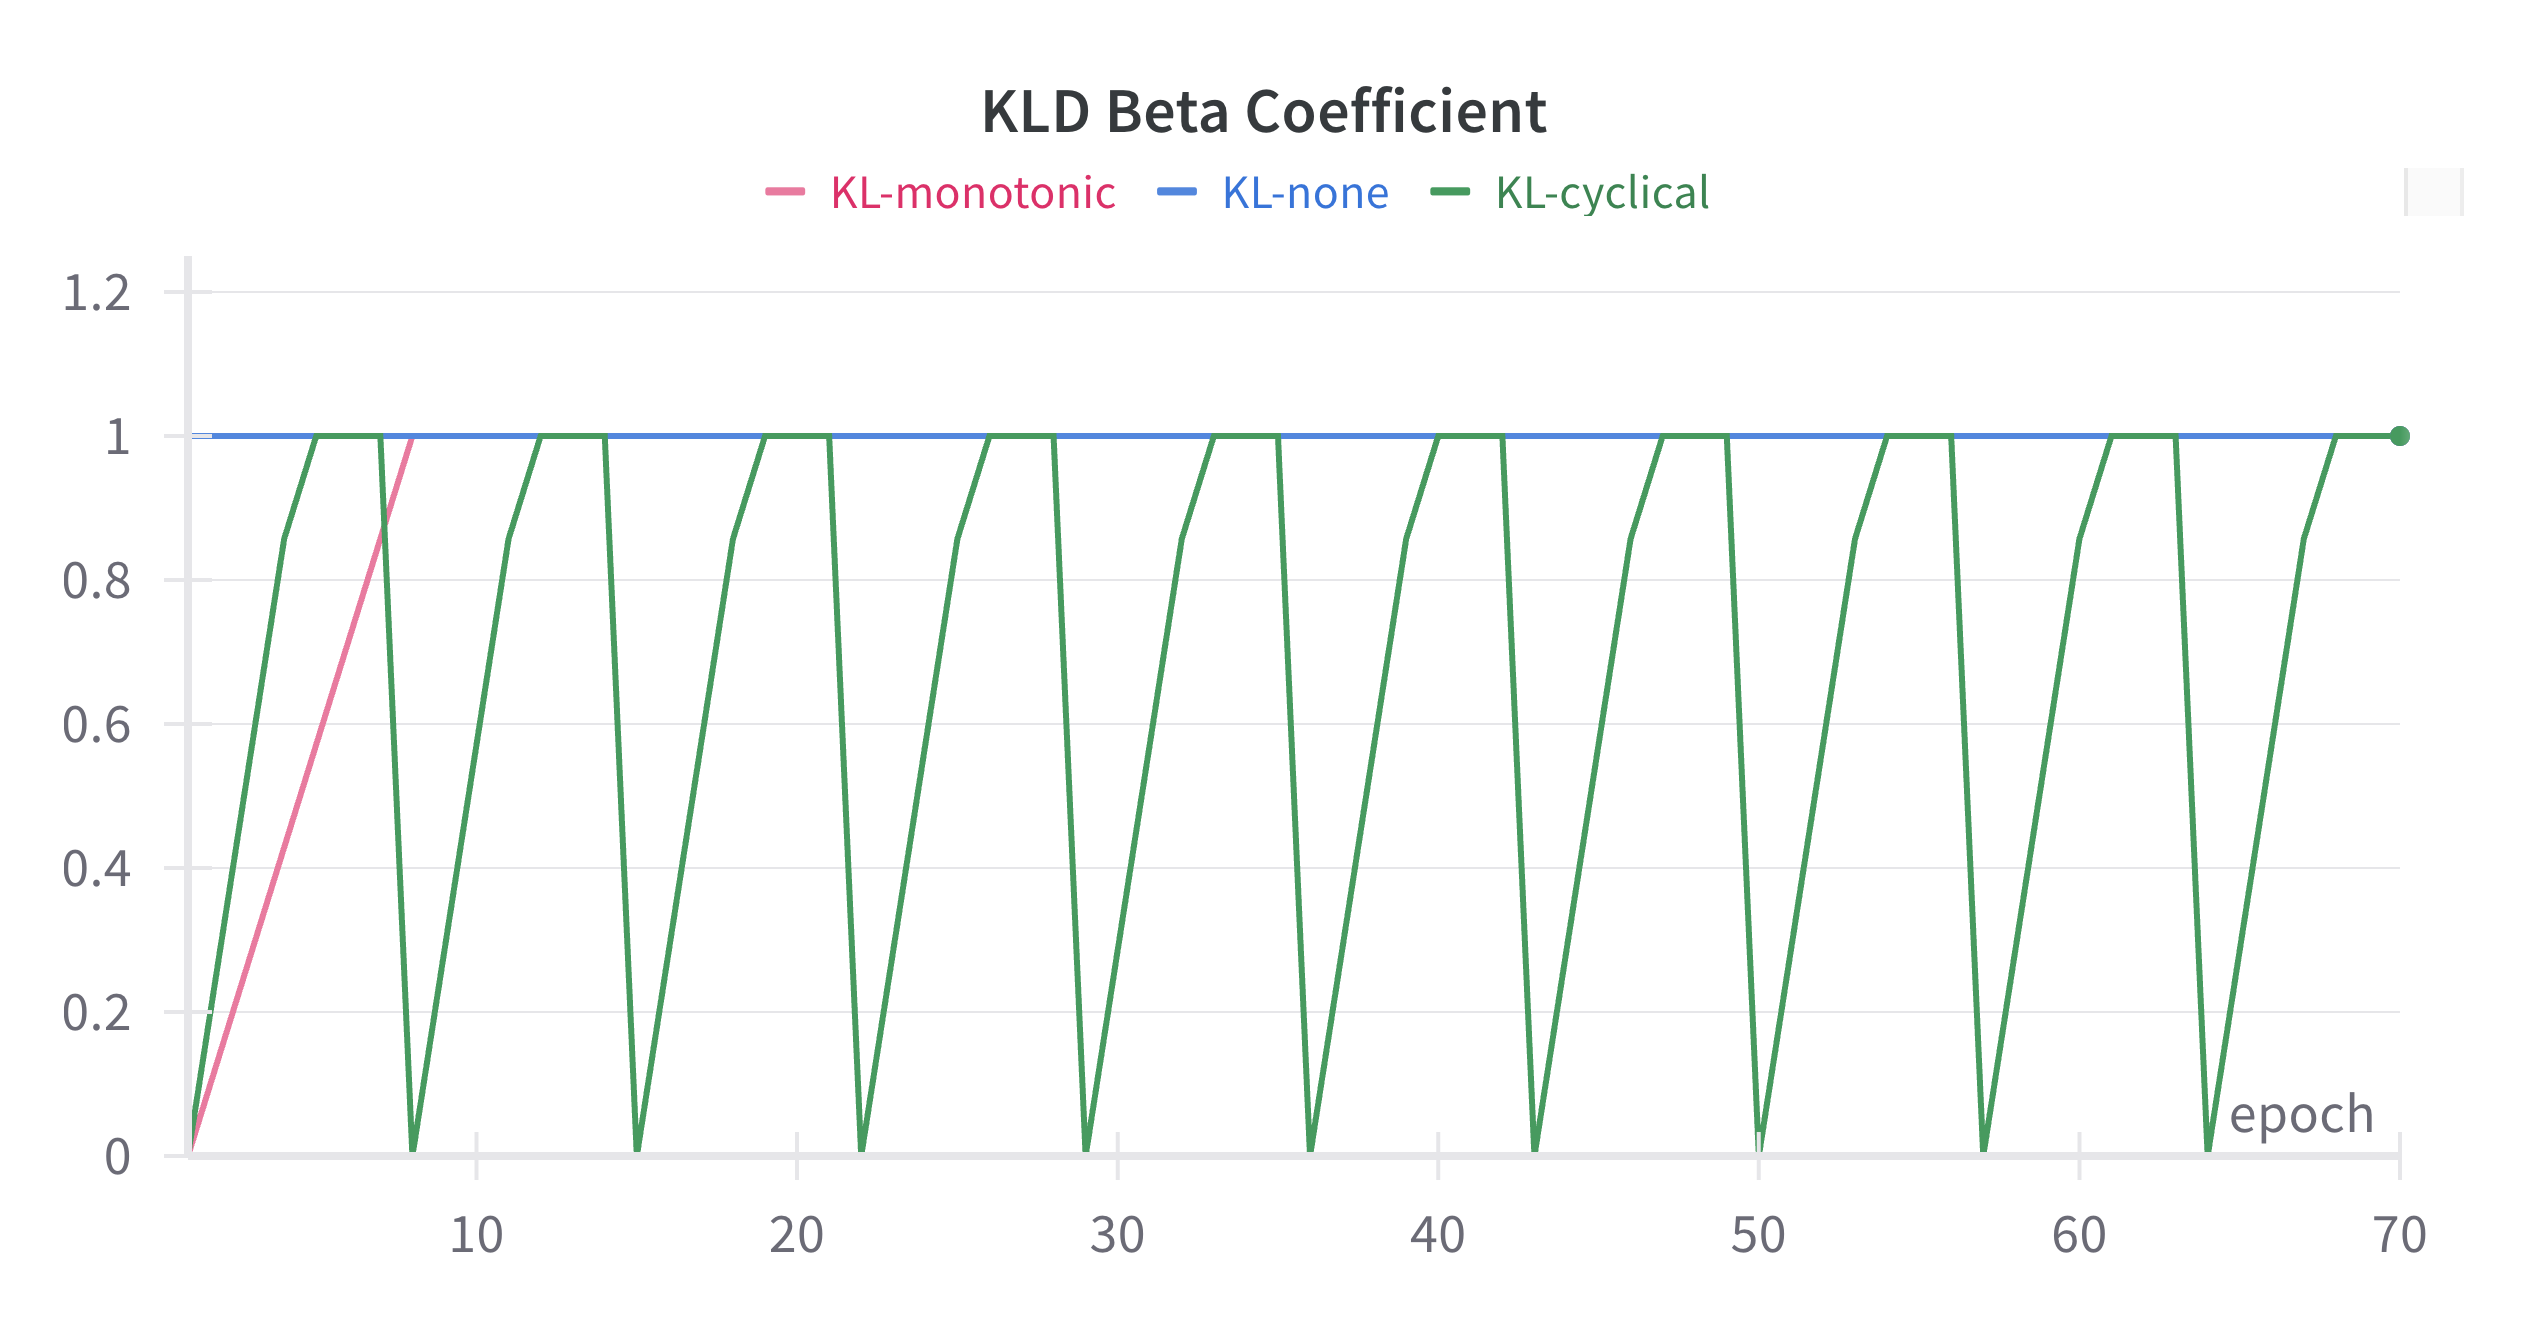
\includegraphics[width=0.95\linewidth]{figures/kl_beta}
\caption{\textbf{The $\beta$ coefficient over training epochs.} In the no annealing setting, $\beta$ is fixed at 1.0. Monotonic annealing linearly increases $\beta$ from 0 to 1. Cyclical annealing linearly increases $\beta$ to 1.0, holds it for half of the cycle, and then resets to 0 to start a new cycle.}
\label{fig:klbeta}
\end{figure}

\begin{figure}[H]
\centering
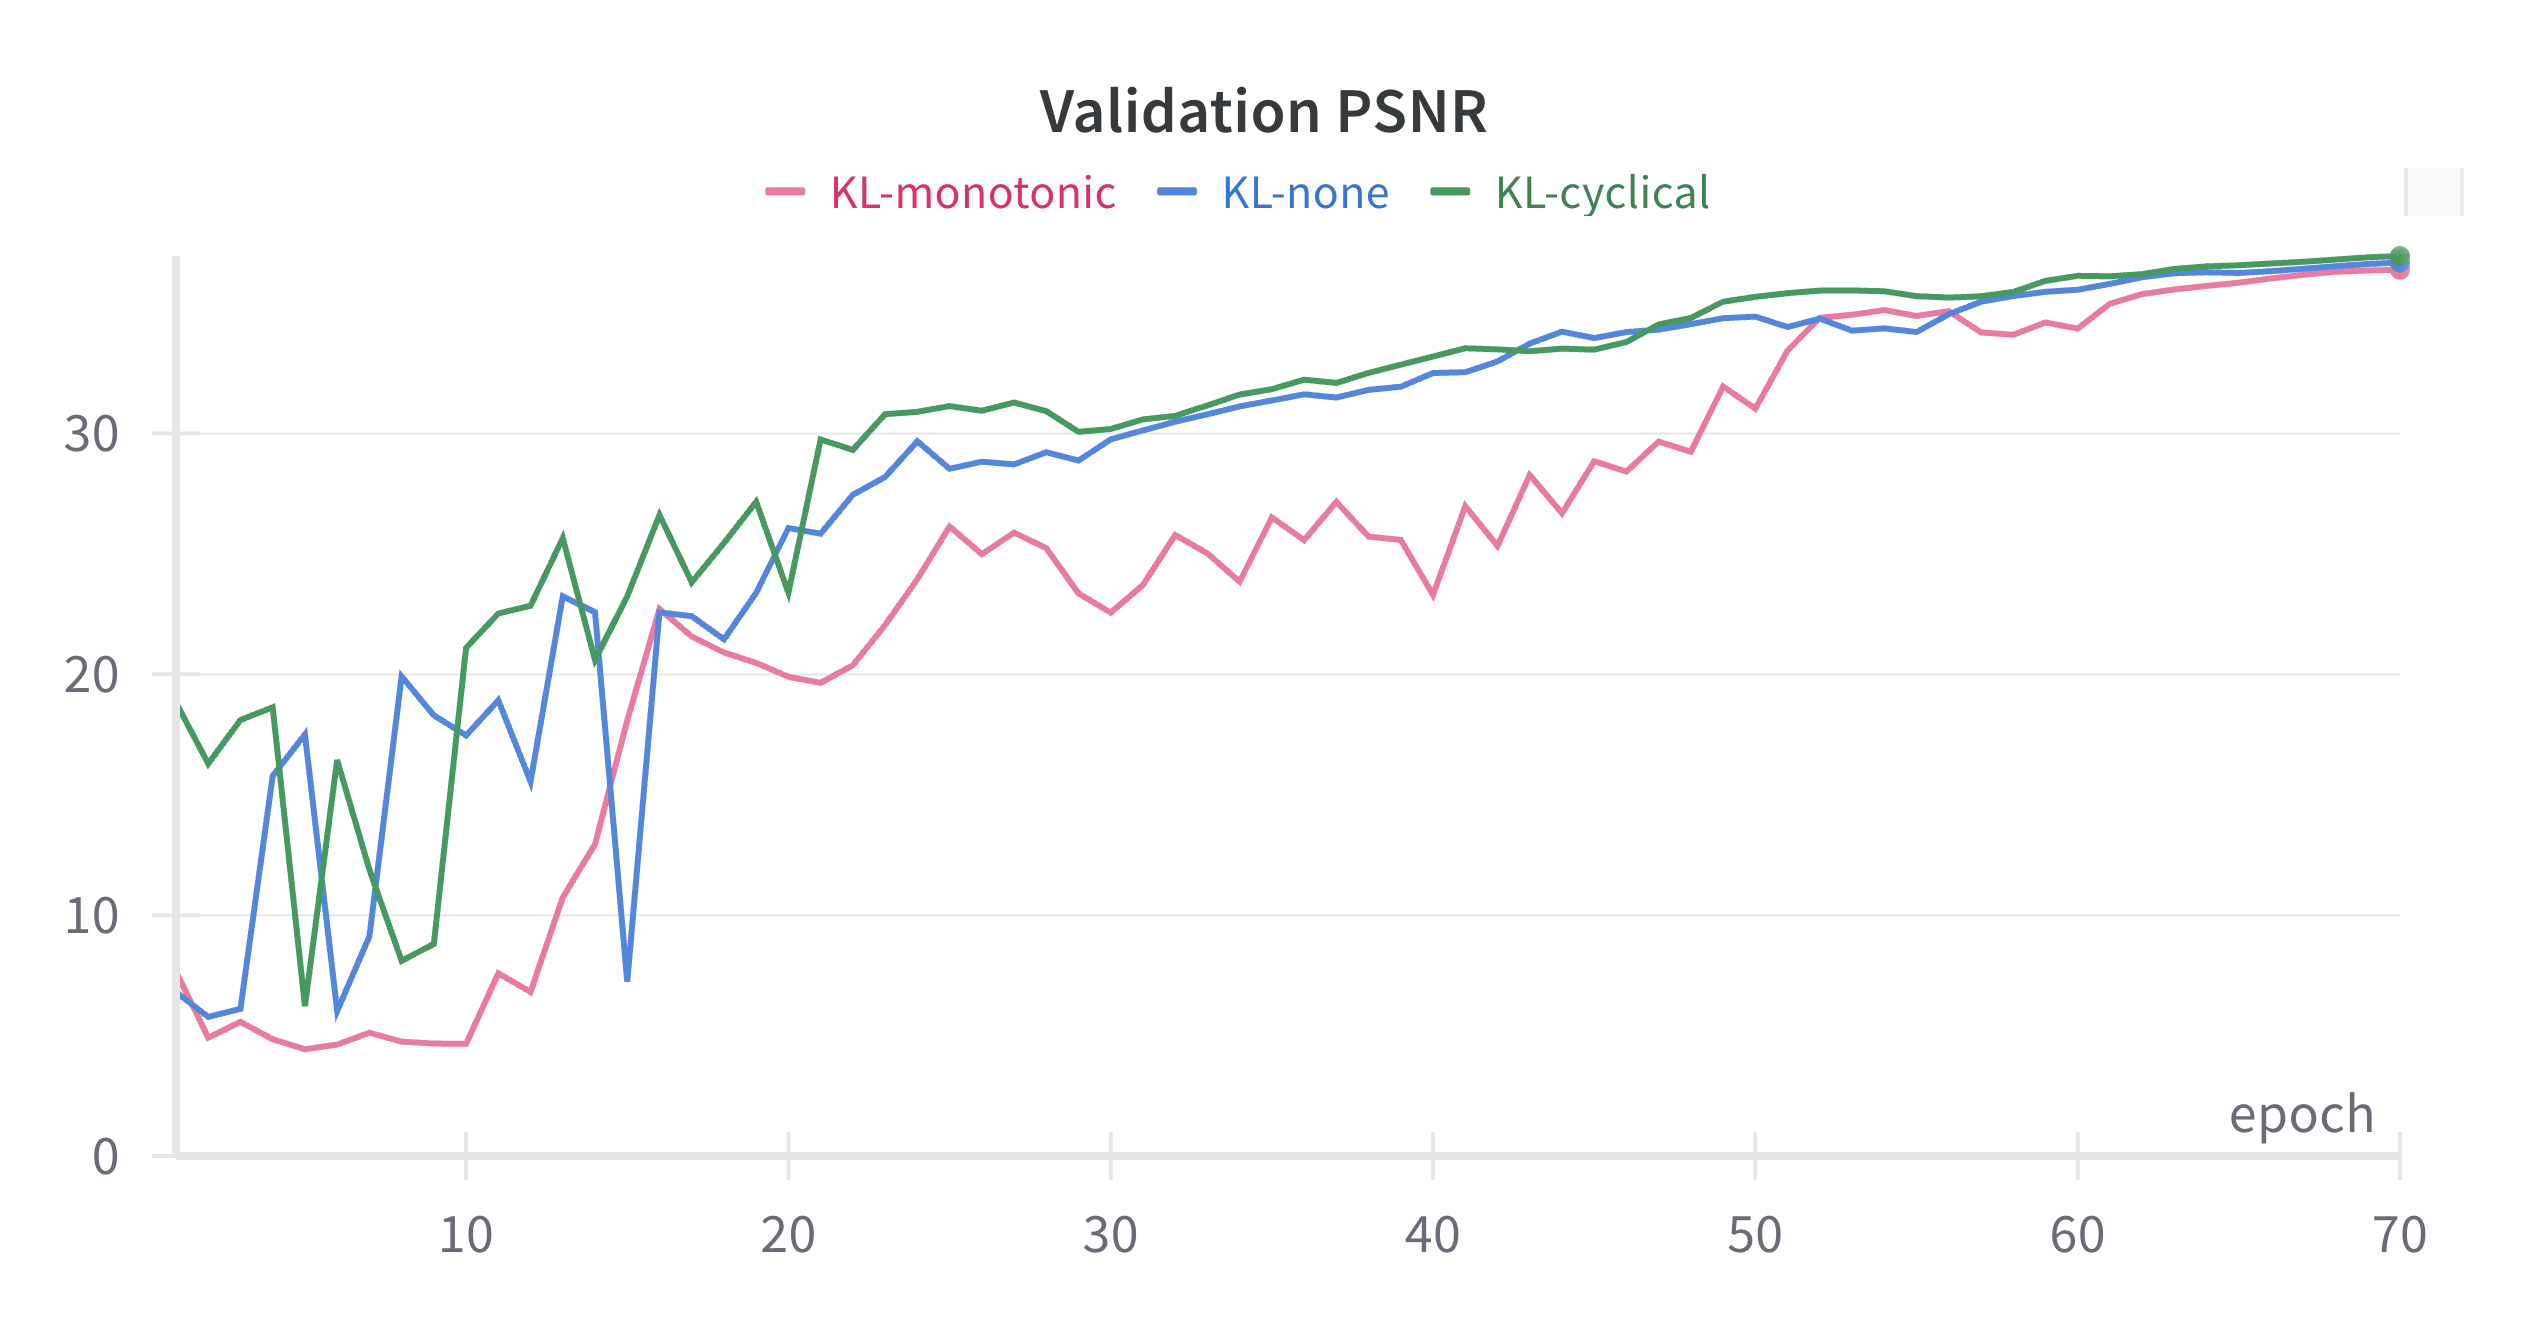
\includegraphics[width=0.95\linewidth]{figures/kl_val_psnr}
\caption{\textbf{Validation PSNR for each annealing method.} Cyclical annealing achieves the best performance with a peak PSNR of 37.37.}
\label{fig:klvalpsnr}
\end{figure}

\begin{figure}[H]
\centering
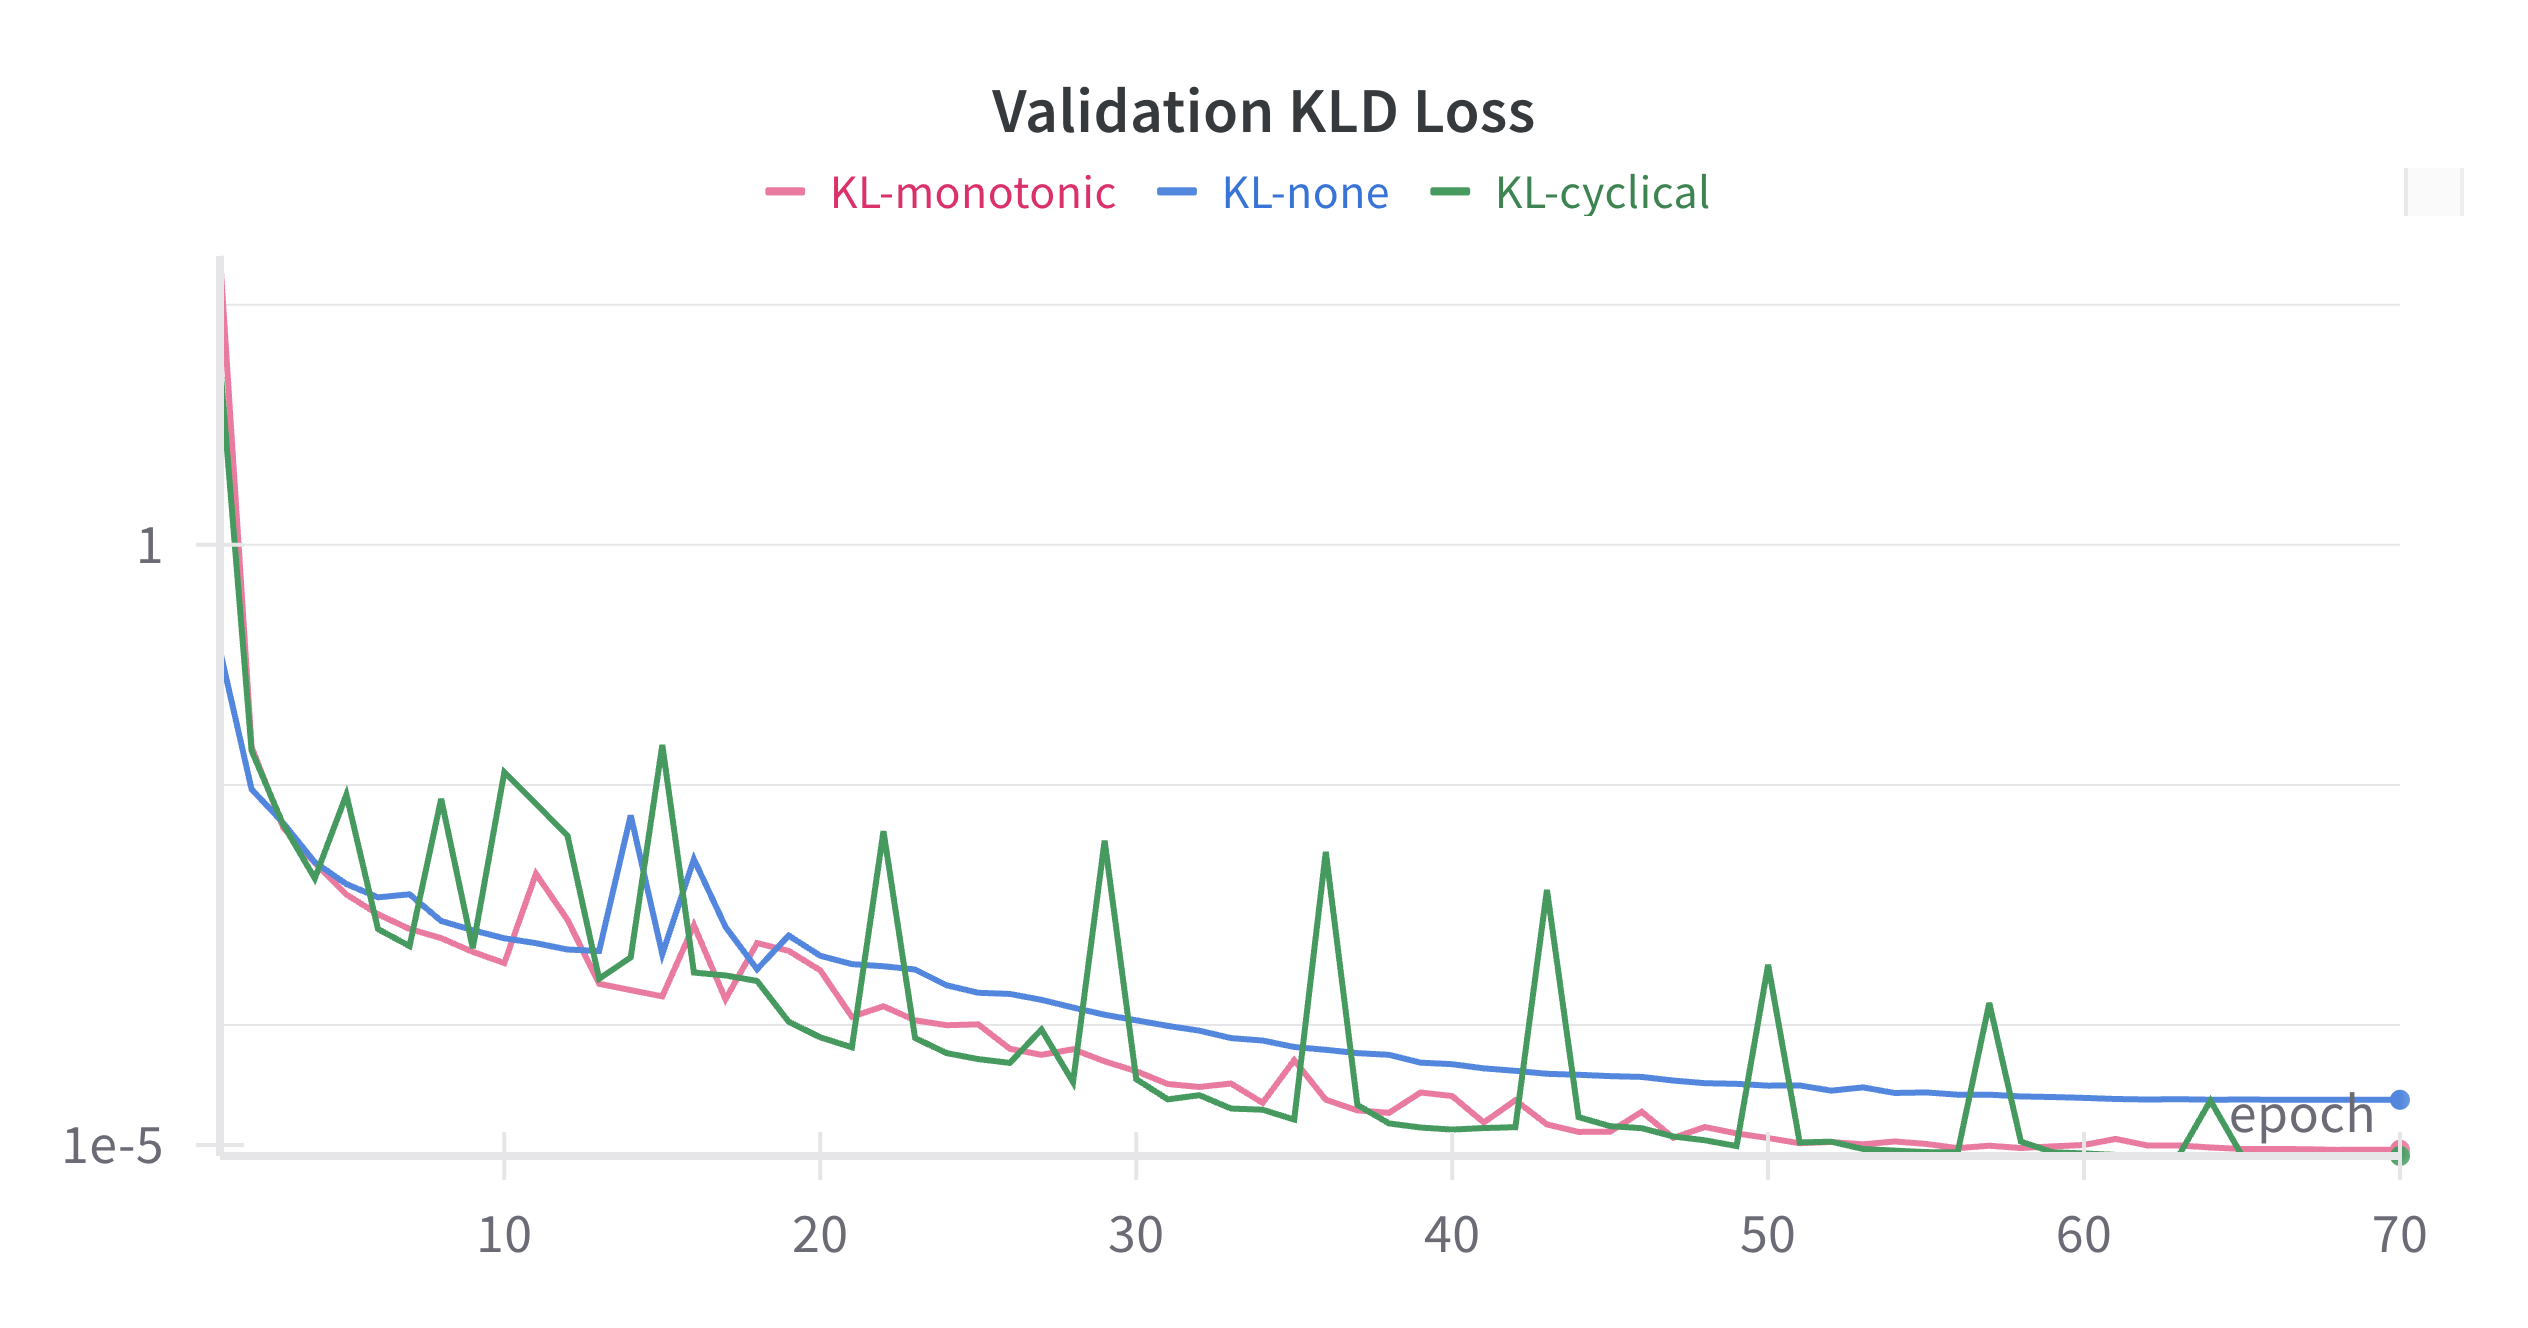
\includegraphics[width=0.95\linewidth]{figures/val_kl_KLD}
\caption{\textbf{Validation KLD across annealing methods.} The KLD for cyclical annealing spikes periodically due to the sudden drop in $\beta$, allowing the model to re-encode diverse latent information.}
\label{fig:valklkld}
\end{figure}

\begin{figure}[H]
\centering
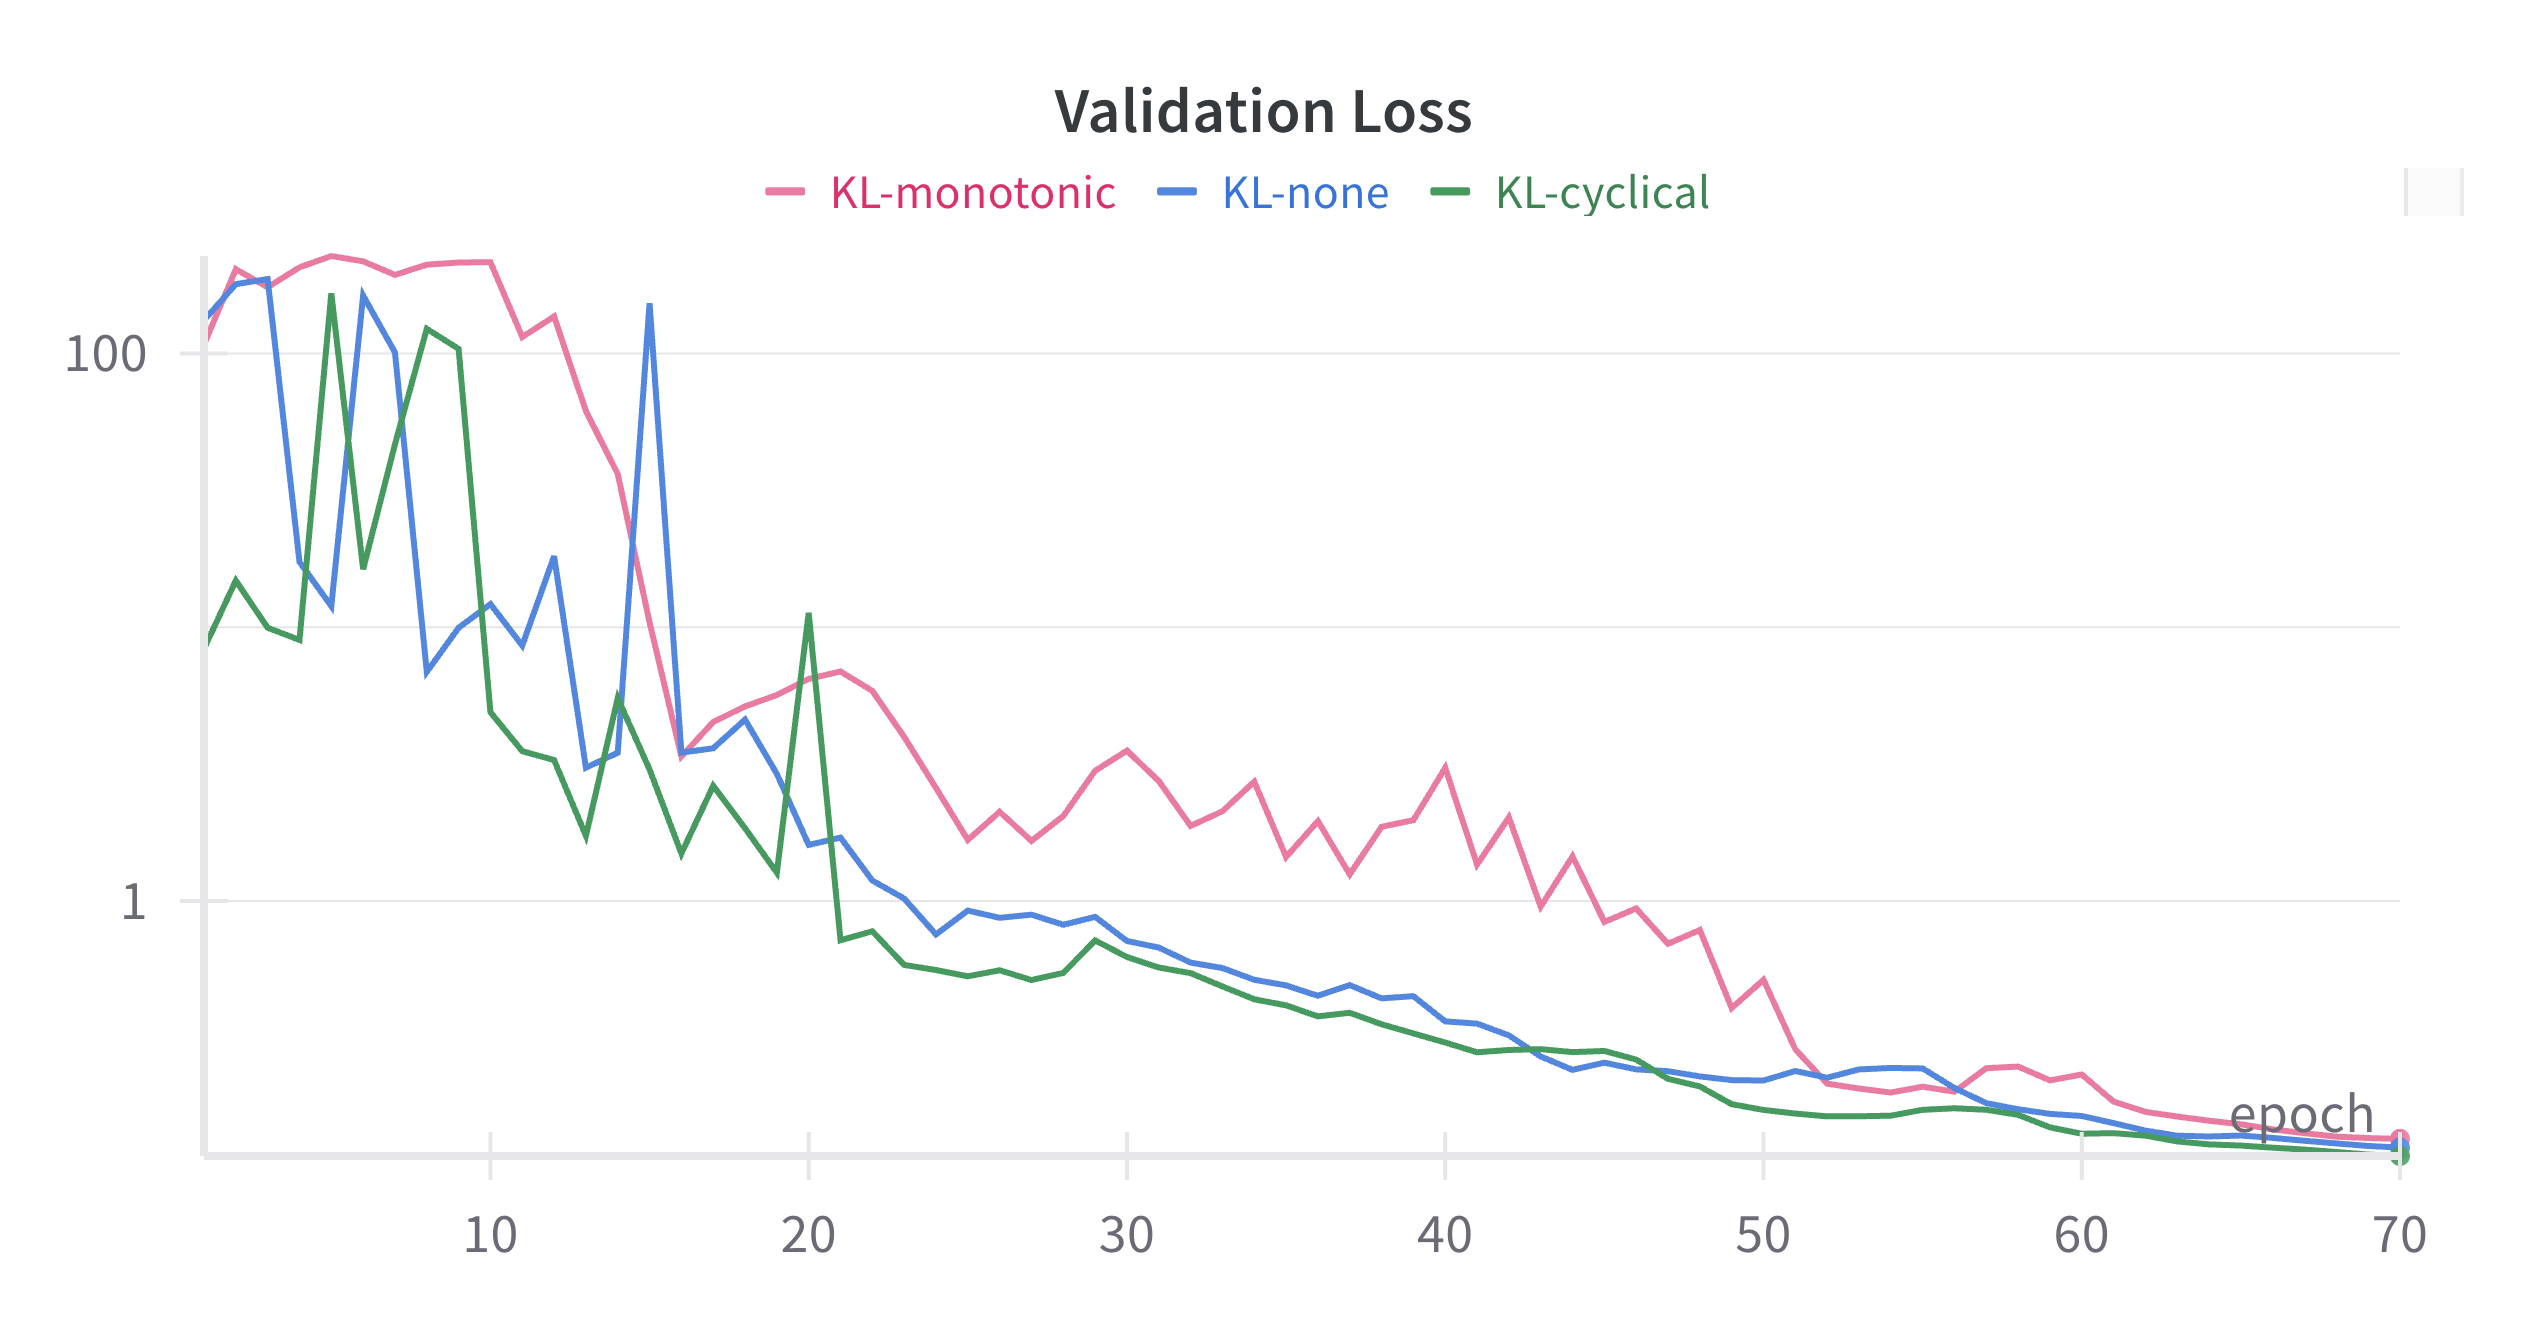
\includegraphics[width=0.95\linewidth]{figures/val_kl_loss}
\caption{\textbf{Total validation loss.} Cyclical annealing consistently achieves the lowest overall loss.}
\label{fig:valklloss}
\end{figure}

\begin{figure}[H]
\centering
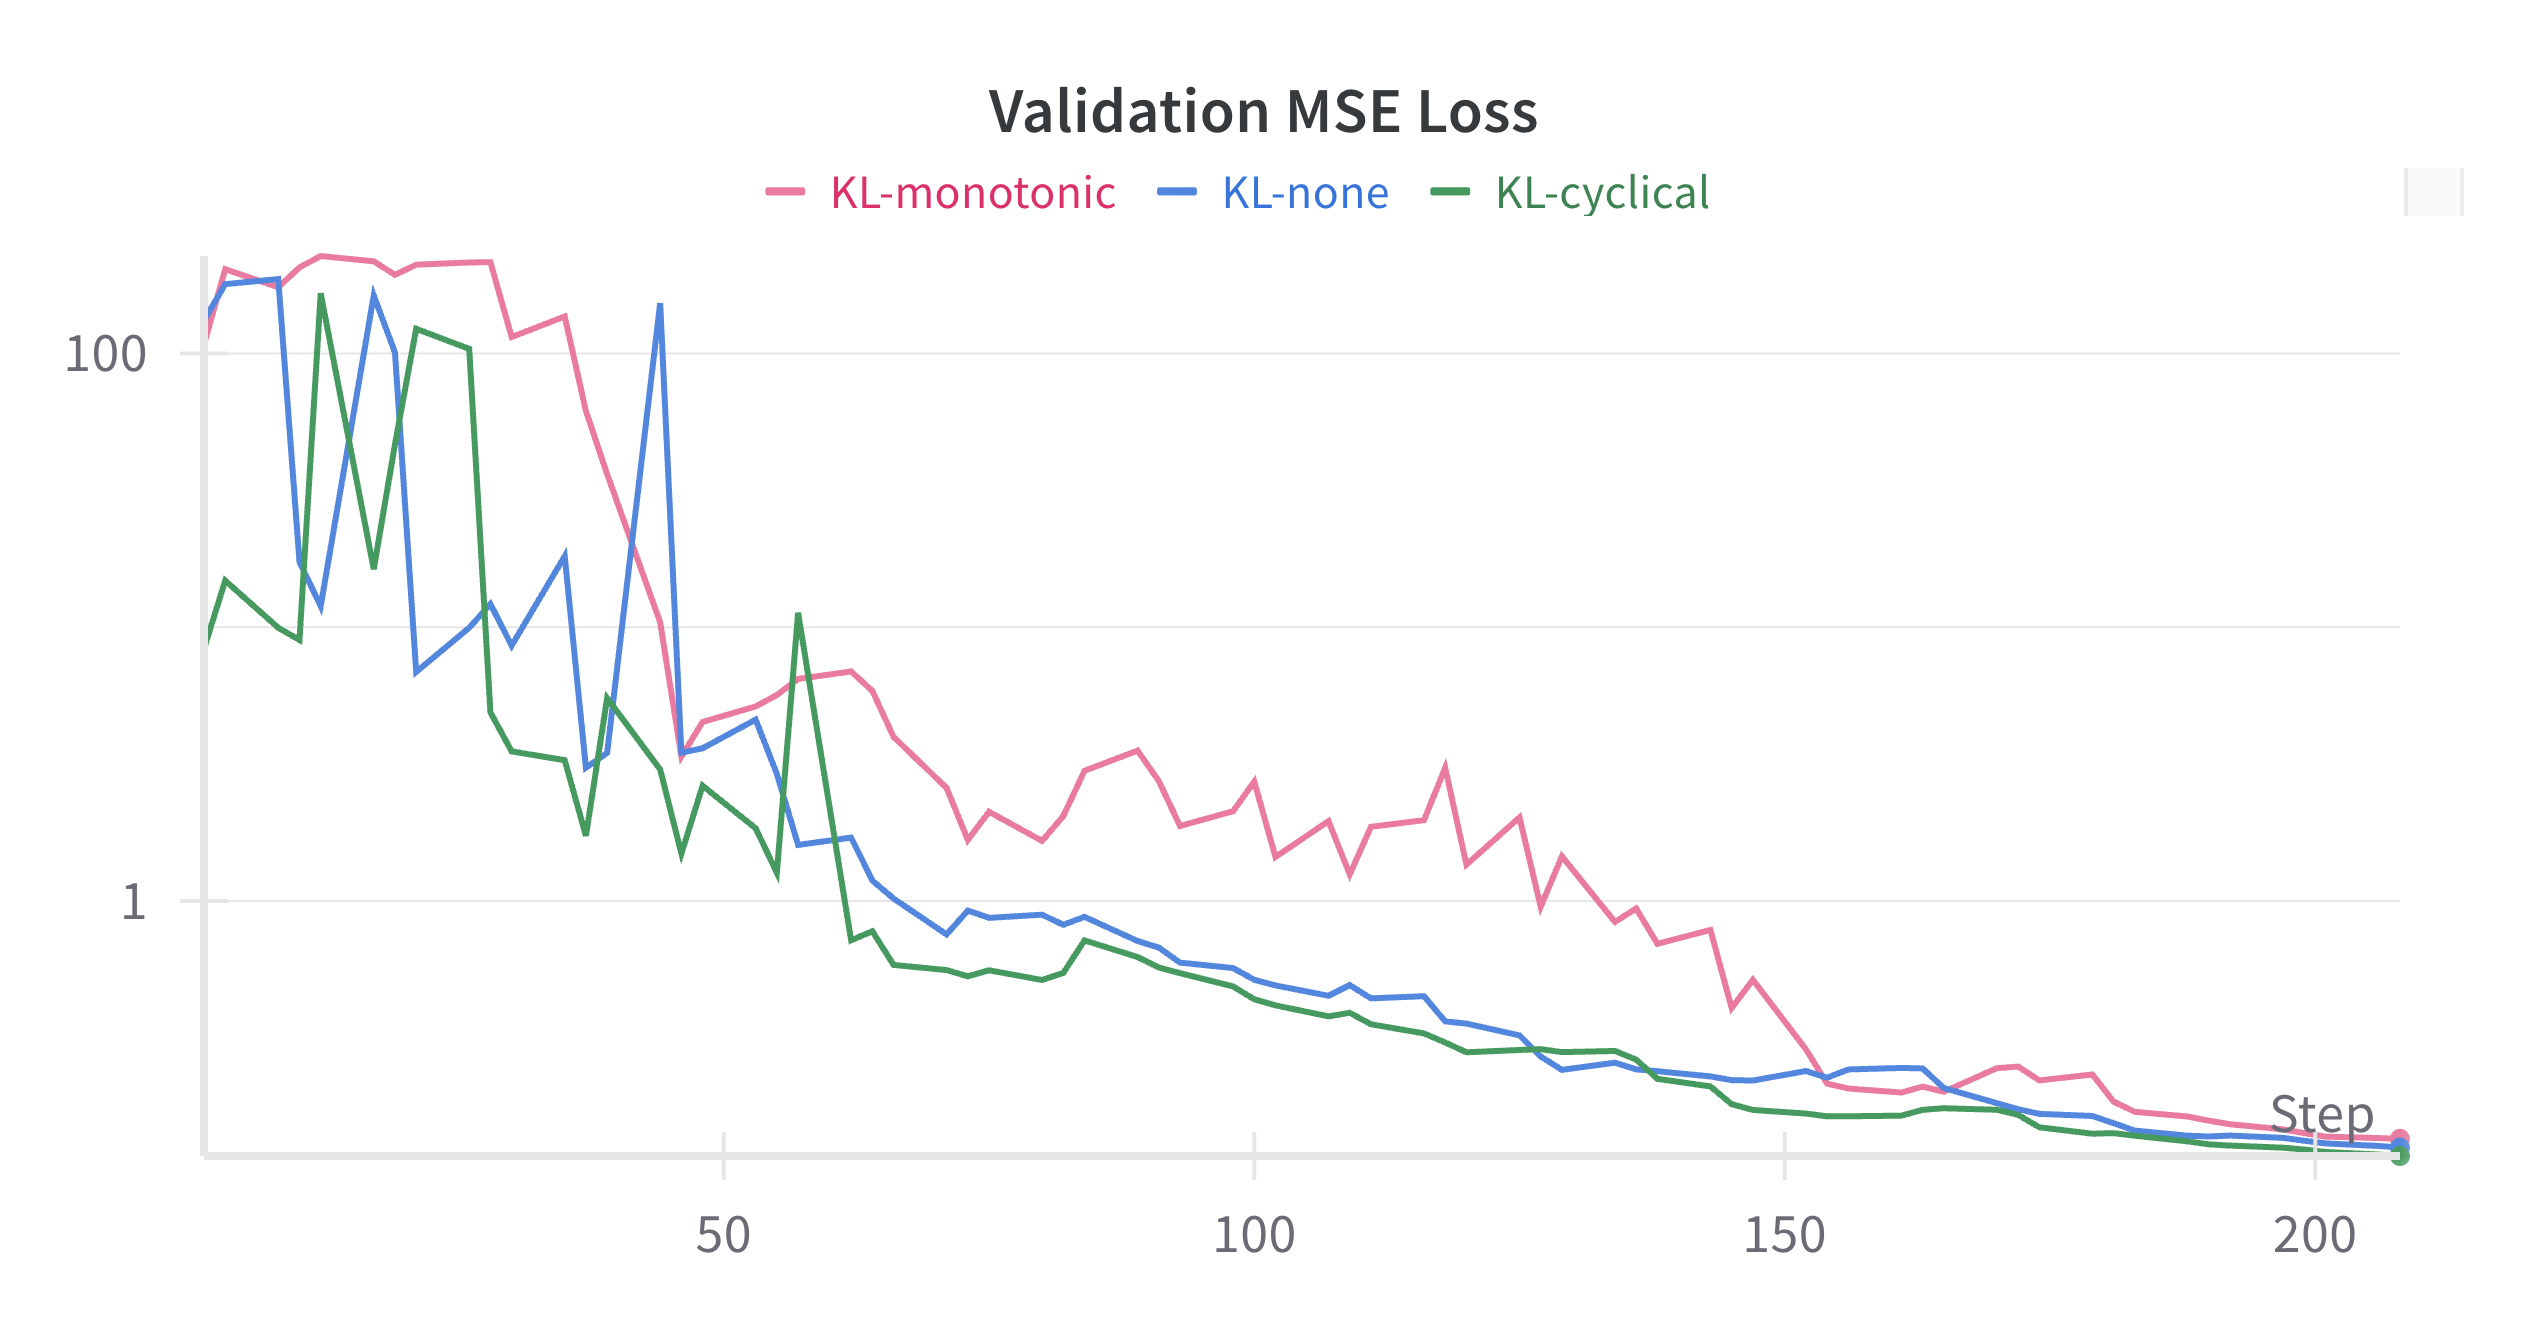
\includegraphics[width=0.95\linewidth]{figures/val_kl_mse}
\caption{\textbf{Validation MSE loss.} The cyclical annealing strategy leads to the lowest reconstruction error.}
\label{fig:valklmse}
\end{figure}

\begin{table}[H]
\centering
\caption{\textbf{Validation PSNR comparison across different KL annealing strategies.} Cyclical annealing achieves the highest PSNR, indicating superior reconstruction performance.}
\begin{tabular}{ccc}
\toprule
\textbf{Cyclical} & \textbf{No Annealing} & \textbf{Monotonic} \\
\midrule
\textbf{37.37368} & 37.10110 & 36.80298 \\
\bottomrule
\end{tabular}
\label{tab:psnr_kl_annealing}
\end{table}

These results are consistent with the findings of \cite{fu2019cyclical}, demonstrating that cyclical annealing effectively prevents KL collapse while enhancing both reconstruction fidelity and latent utilization.

\subsection{Teacher Forcing Ratio}

Through empirical analysis, I observed that disabling teacher forcing entirely (i.e., setting the initial ratio to 0) led to unstable training and \texttt{NaN} loss in the early stages. This instability stems from the accumulation of errors during auto-regressive generation, especially when the model is not yet trained to handle compounding prediction errors.

As shown in \autoref{fig:tfr}, I implemented a scheduled reduction strategy where the teacher forcing ratio begins at 1.0 and remains constant for the first 10 epochs. After this initial stabilization period, the ratio decreases linearly by 0.1 each epoch until it reaches 0, allowing the model to gradually adapt to its own predictions.

This phenomenon is also reflected in \autoref{fig:klvalpsnr}, where the PSNR occasionally drops to very low values during the first 10 epochs when teacher forcing ratio is high. However, as training progresses and teacher forcing is gradually reduced, the model stabilizes, and the PSNR consistently improves across all three KL annealing strategies.

These results indicate that a scheduled reduction of teacher forcing helps prevent error accumulation in the early stages while encouraging stronger temporal generalization in later stages of training. The gradual transition from ground truth inputs to model-generated inputs proves crucial for achieving stable convergence in sequence prediction tasks.

\begin{figure}[H]
\centering
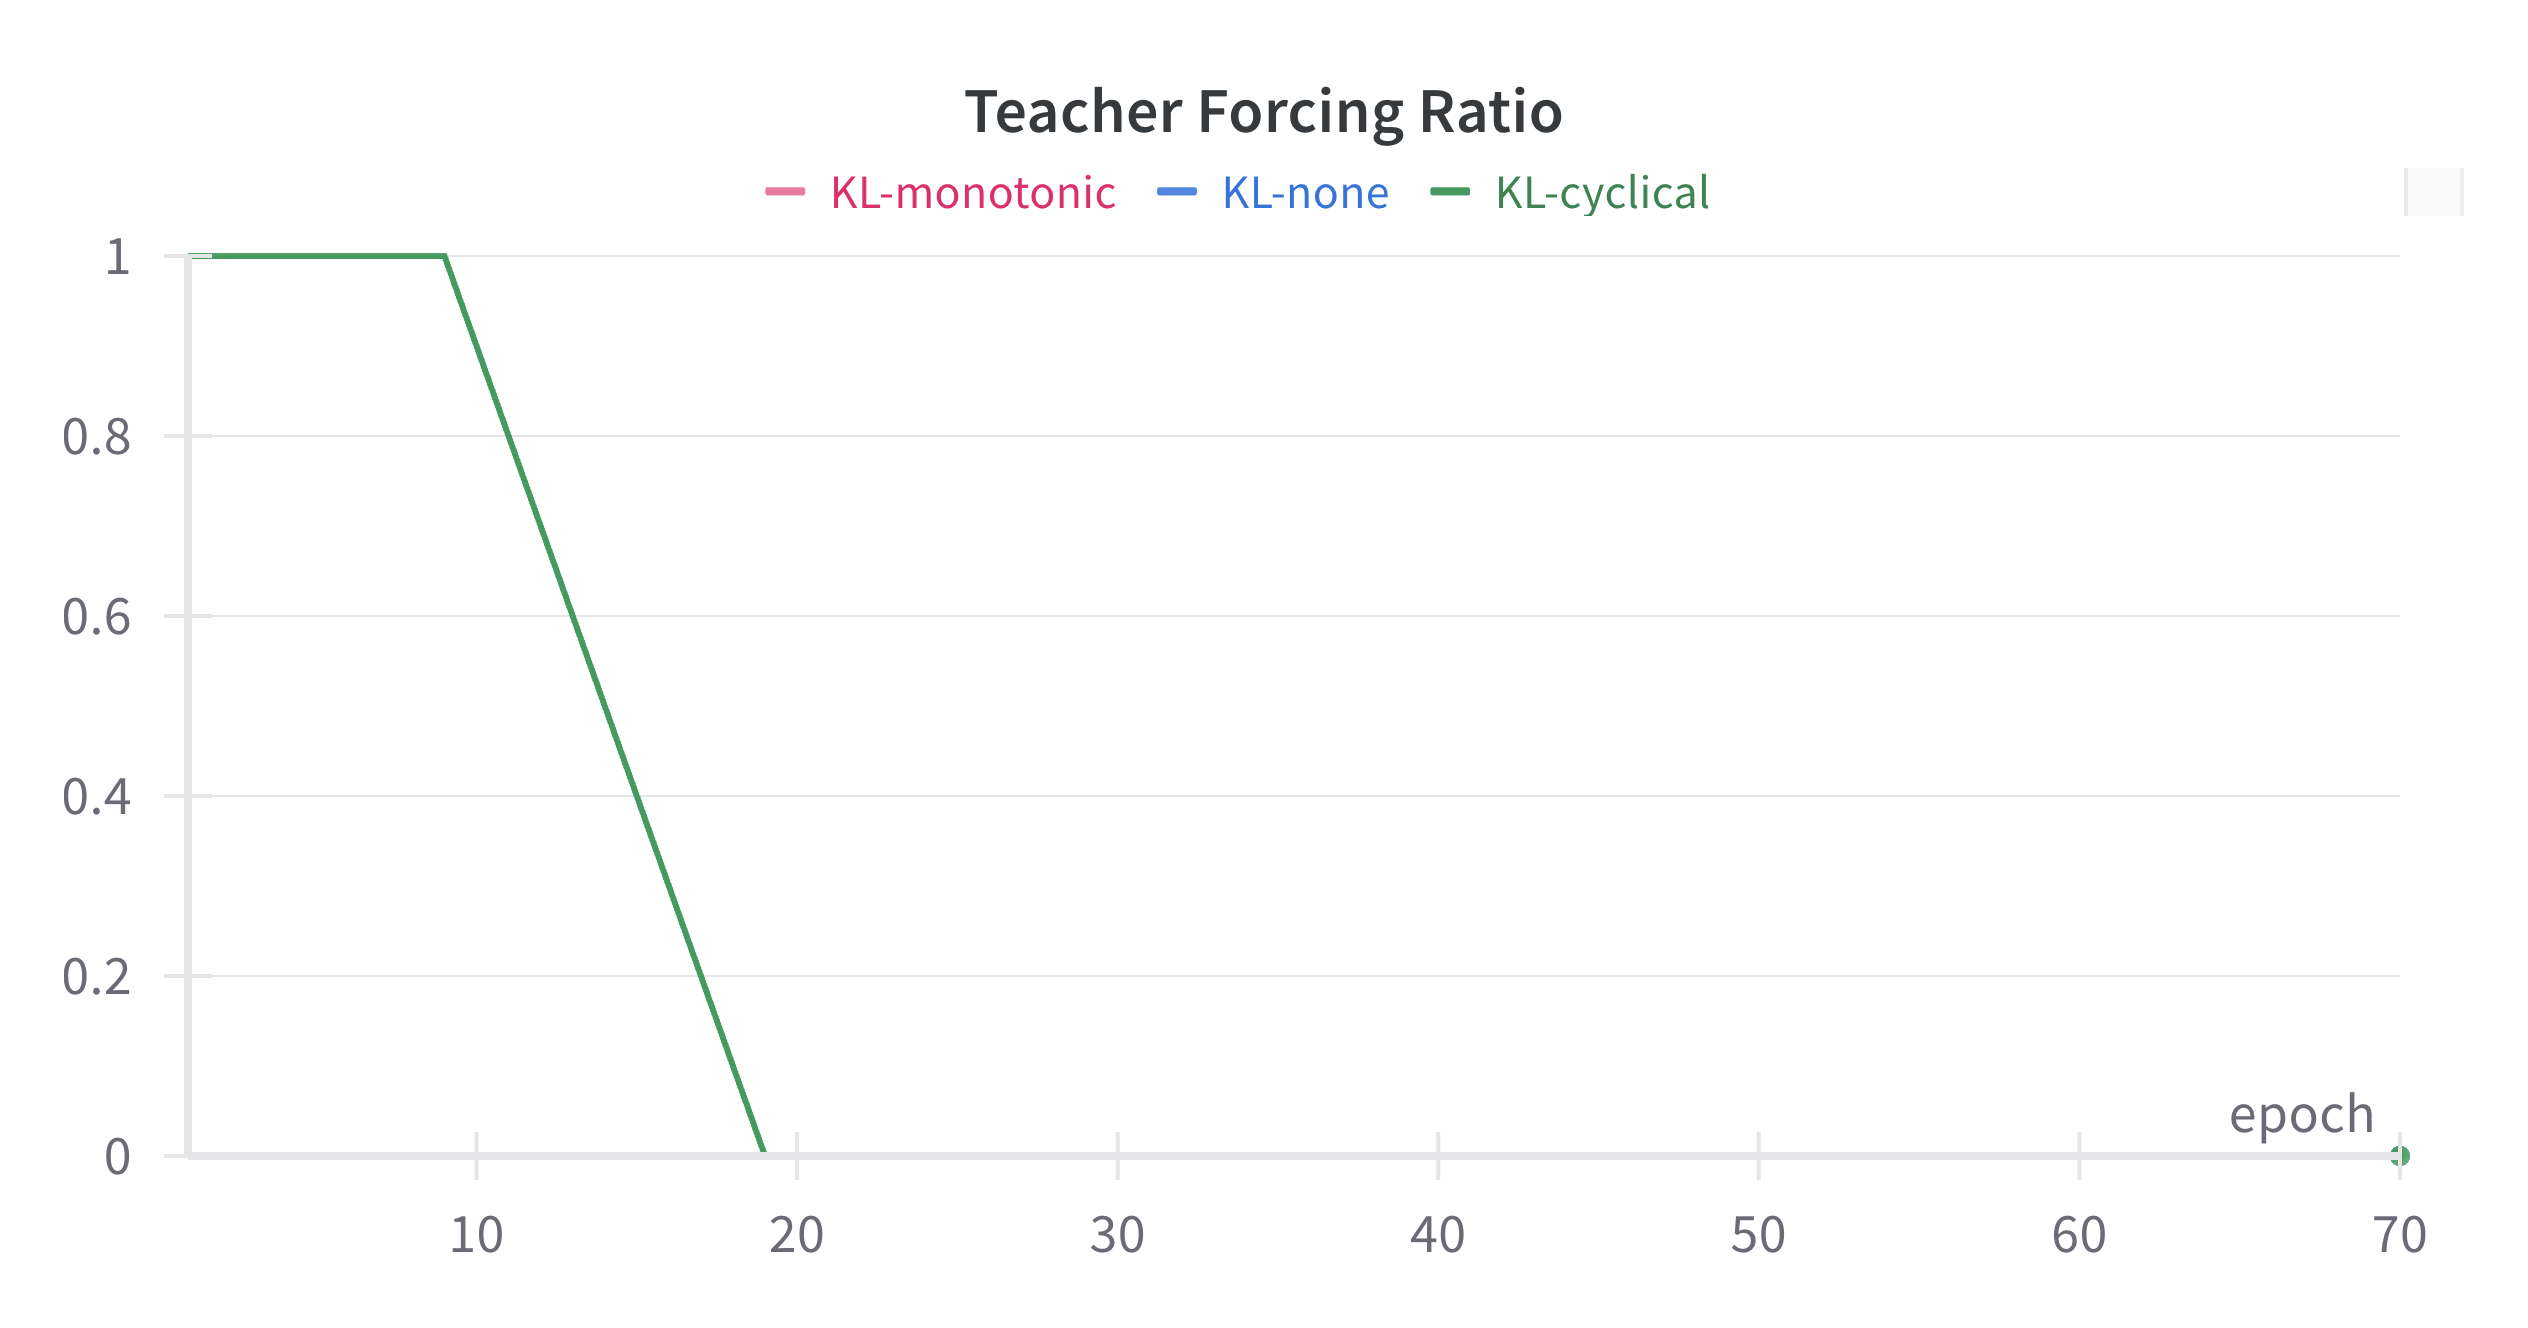
\includegraphics[width=0.95\linewidth]{figures/tfr}
\caption{\textbf{The teacher forcing ratio over time.} The ratio remains at 1.0 for the first 10 epochs to establish model stability, then gradually decreases by 0.1 per epoch until reaching 0.}
\label{fig:tfr}
\end{figure}



\subsection{Per-frame PSNR Analysis}

To better understand the temporal consistency and reconstruction fidelity of the trained model, I analyzed the PSNR value for each frame in the validation sequence. \autoref{fig:val70framepsnr} shows the per-frame PSNR curve for the model trained over 70 epochs using cyclical KL annealing.

The model demonstrates relatively stable reconstruction across most of the 630-frame sequence, maintaining PSNR values between 36 dB and 38.5 dB. However, there are several notable dips in performance. Specifically, frames between 170–190 and 400–500 experience significant PSNR degradation. These drops indicate that the model struggles with maintaining quality in longer-term predictions, likely due to compounding errors in the auto-regressive generation process.

These findings support the necessity of techniques such as teacher forcing in the early training phase. The per-frame evaluation highlights that some temporal regions remain challenging even for a well-trained model.

\begin{figure}[H]
\centering
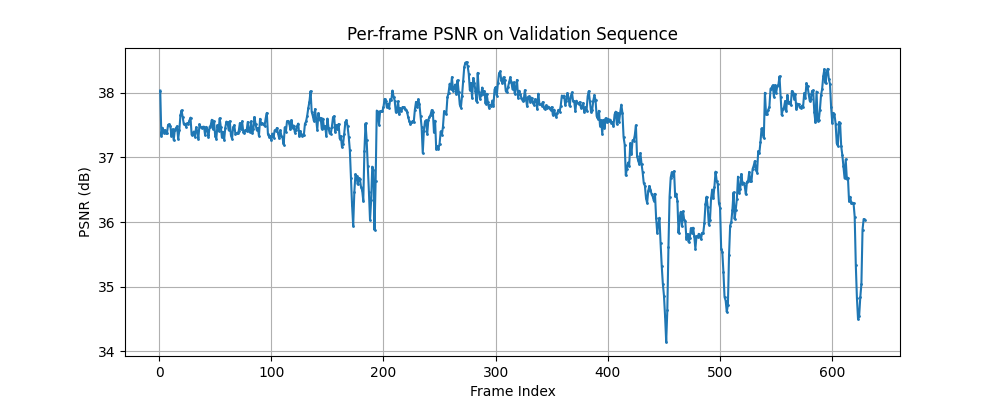
\includegraphics[width=0.95\linewidth]{figures/val_70_frame_psnr}
\caption{\textbf{Per-frame PSNR of the model trained for 70 epochs.} The model achieves an overall stable reconstruction performance, but certain segments (e.g., frames 170–190 and 400–500) exhibit noticeable PSNR drops due to error accumulation in long-term prediction.}
\label{fig:val70framepsnr}
\end{figure}

\subsection{Additional Training Details for Submission}

To further enhance model performance, I trained a second model using the same cyclical KL annealing strategy but extended the training to 140 epochs. This resulted in a validation PSNR of 38.2362 and a public test PSNR of 36.0714. In comparison, the model trained for only 70 epochs achieved a validation PSNR of 37.3737 and a public test PSNR of 35.0846. The extended training notably improved generalization and reduced the PSNR drop across difficult frames.

\begin{figure}[H]
\centering
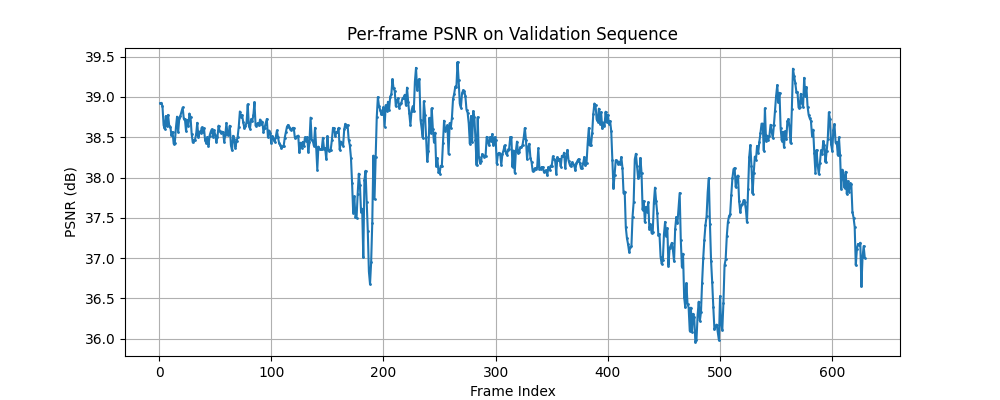
\includegraphics[width=0.95\linewidth]{figures/val_140_frame_psnr}
\caption{\textbf{Per-frame PSNR of the model trained for 140 epochs.} Compared to the 70-epoch model, the extended training achieves consistently higher PSNR across most frames, indicating improved long-term consistency and reconstruction fidelity.}
\label{fig:val140framepsnr}
\end{figure}

The per-frame PSNR analysis of the 140-epoch model shows significant improvements especially in the previously problematic regions (frames 170-190 and 400-500). The overall PSNR curve is more stable with fewer sharp drops, indicating better temporal consistency throughout the sequence. This demonstrates that with extended training, the model becomes more robust to error accumulation in long-term predictions.

\section{Conclusion}
In this lab, I implemented a conditional VAE for video frame prediction using pose information. Through experimentation with different training strategies, I found that:

\begin{enumerate}
    \item Cyclical KL annealing effectively prevents KL vanishing and leads to better model performance compared to monotonic annealing or no annealing. This aligns with the findings in \cite{fu2019cyclical}.
    \item Teacher forcing with a gradual decay strategy helps stabilize early training while allowing the model to learn to handle accumulated errors during inference.
    \item Extended training (140 epochs) significantly improves model performance, especially for long-term prediction stability.
\end{enumerate}

The results demonstrate the importance of proper regularization and training strategies when working with VAEs for sequential data generation tasks. By combining cyclical KL annealing and teacher forcing, we achieved high-quality frame prediction with PSNR values above 38 dB on the validation set and above 36 dB on the public test set.

These findings highlight that addressing the inherent challenges in VAE training (particularly KL vanishing) and sequential prediction (error accumulation) can lead to significant improvements in performance for video generation tasks.

\printbibliography
\end{document}